\documentclass[../mathNotesPreamble]{subfiles}

\providecommand{\relscalefact}{1.4}
\begin{document}
\relscale{\relscalefact}
  \section{3.1: Summaries for Symmetric Distributions}
  \begin{defn*}
    Given a collection of data $\set{x_1,x_2,\dots,x_n}$, the \textbf{mean} of the data is the arithmetic mean:
      \[\bar{x}=\frac{x_1}{n}+\frac{x_2}{n}+\dots+\frac{x_n}{n}=\frac{1}{n}\sum_{i=1}^n x_i\]
  \end{defn*}
  \vspace*{0.5\baselineskip}

  \begin{ex*}
    An instructor at Peoria Junior College in Illinois collected data from two classes, including the students’ ACT scores. Below is the distribution of self-reported ACT scores for one statistics class:
  \end{ex*}
  \vspace*{0.5\baselineskip}
  \begin{center}
    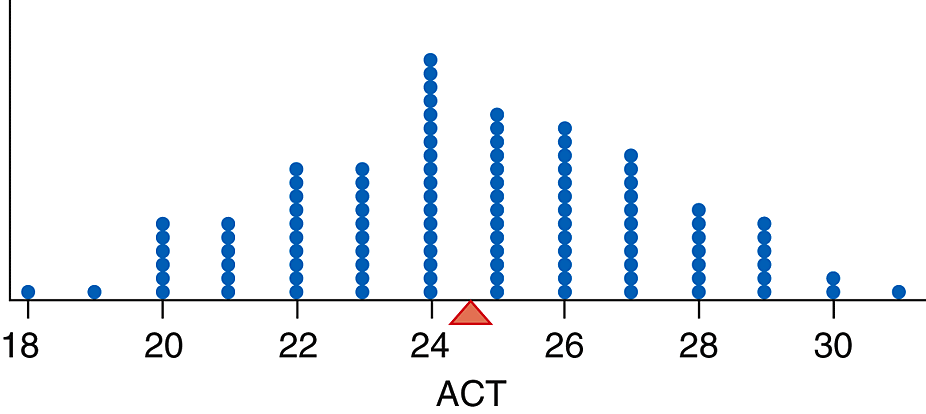
\includegraphics[width=0.6\linewidth]{images/math211_figure_3p2}
  \end{center}
  \vspace*{\stretch{1}}

  \begin{ex*}
    The winnings of the top-ranked professional tennis players in the 2018 season are given in the graph below:
  \end{ex*}
  \vspace*{0.5\baselineskip}
  \begin{center}
    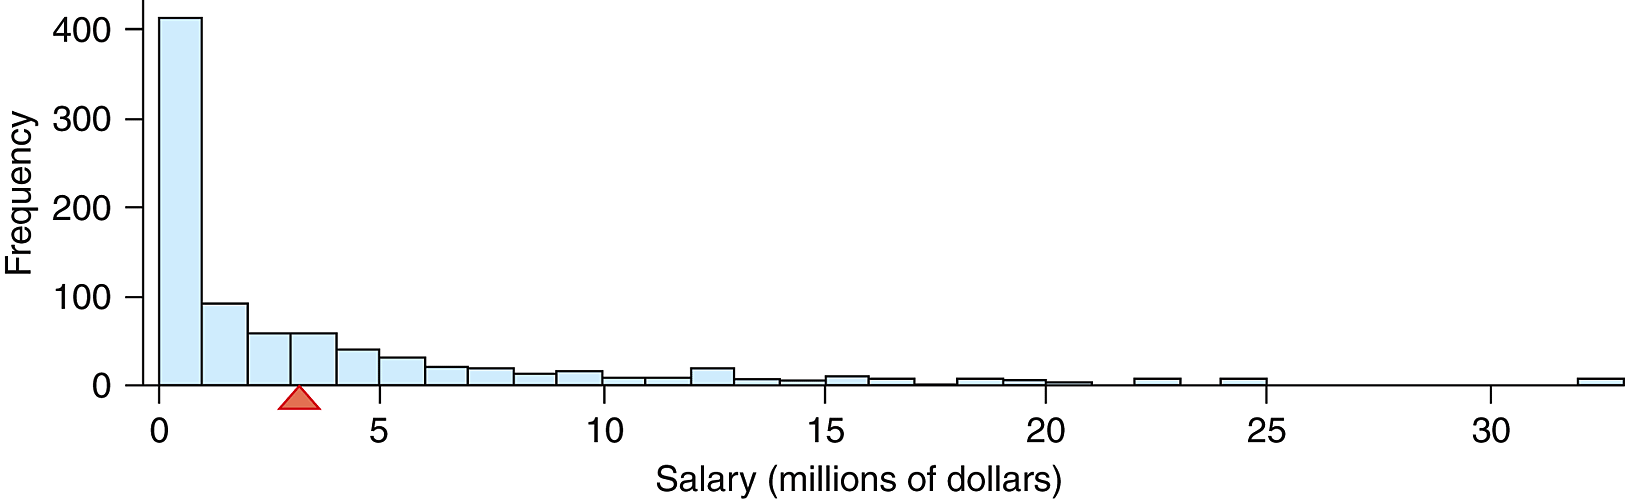
\includegraphics[width=0.6\linewidth]{images/math211_figure_3p3}
  \end{center}
%  \vspace*{\stretch{1}}
  \pagebreak

  \noindent
  \fbox{\parbox{0.9875\linewidth}{\emph{Note}:
  \begin{itemize}
    \item When the distribution is roughly symmetric, the mean represents a typical value in the data.
    \item The mean is \emph{not} a good estimate of a typical value of a skewed distribution.
  \end{itemize}}}
  \begin{ex*}
    According to GasBuddy.com (a website that invites people to submit prices at local gas stations), the prices of 1 gallon of regular gas at 12 service stations near the downtown area of Austin, TX, were as follows one winter day in 2018:
    \vspace*{\baselineskip}

    \noindent
    \begin{minipage}{0.4\linewidth}
      \begin{center}
        \begin{tabular}{@{}*{4}{c}@{}}\toprule
          \$2.19 & \$2.19 & \$2.39 & \$2.19 \\
          \$2.24 & \$2.39 & \$2.27 & \$2.29 \\
          \$2.17 & \$2.29 & \$2.30 & \$2.29 \\\bottomrule
        \end{tabular}
      \end{center}
    \end{minipage}\hspace*{\stretch{1}}
    \begin{minipage}{0.6\linewidth}
      \centering
      \begin{tikzpicture}
        \begin{axis}[
          axis lines=center,
          axis line style={black,->},
          xmin=2.14, xmax=2.41,
          ymin=0,
          ymajorticks=false,
          width=0.9\linewidth,
          height=0.33\linewidth,
          ticklabel style={font=\normalsize,inner sep=0.5pt,fill=white,opacity=1.0, text opacity=1}]
            \foreach \price/\freq in {
              2.17/1,
              2.19/3,
              2.24/1,
              2.27/1,
              2.29/3,
              2.3/1,
              2.39/2
              }{
              \foreach \x in {1,...,\freq}
                \addplot[soldot, mark size=2pt] coordinates{(\price,\x)};
              }
        \end{axis}
      \end{tikzpicture}
    \end{minipage}
    \vspace*{\baselineskip}

    Find the mean price of a gallon of regular gas at these service stations, and interpret the result.
  \end{ex*}
  \pagebreak

  \begin{defn*}
    The \textbf{standard deviation} is a number that measures how far the typical observation is from the mean. For symmetric, unimodal distributions, a majority of the data is within one standard deviation of the mean. The standard deviation is given by
      \[s=\sqrt{\frac{\sum \parens{x_i-\bar{x}}^2}{\nmo}}\]
    \vspace*{-0.75\baselineskip}
  \end{defn*}

  \begin{ex*}
    The histograms below show daily high temperatures in degrees Fahrenheit recorded over one year in Provo, Utah (left), and San Francisco, California (right). Which city do we expect to have a higher standard deviation?
  \end{ex*}
  \begin{center}
    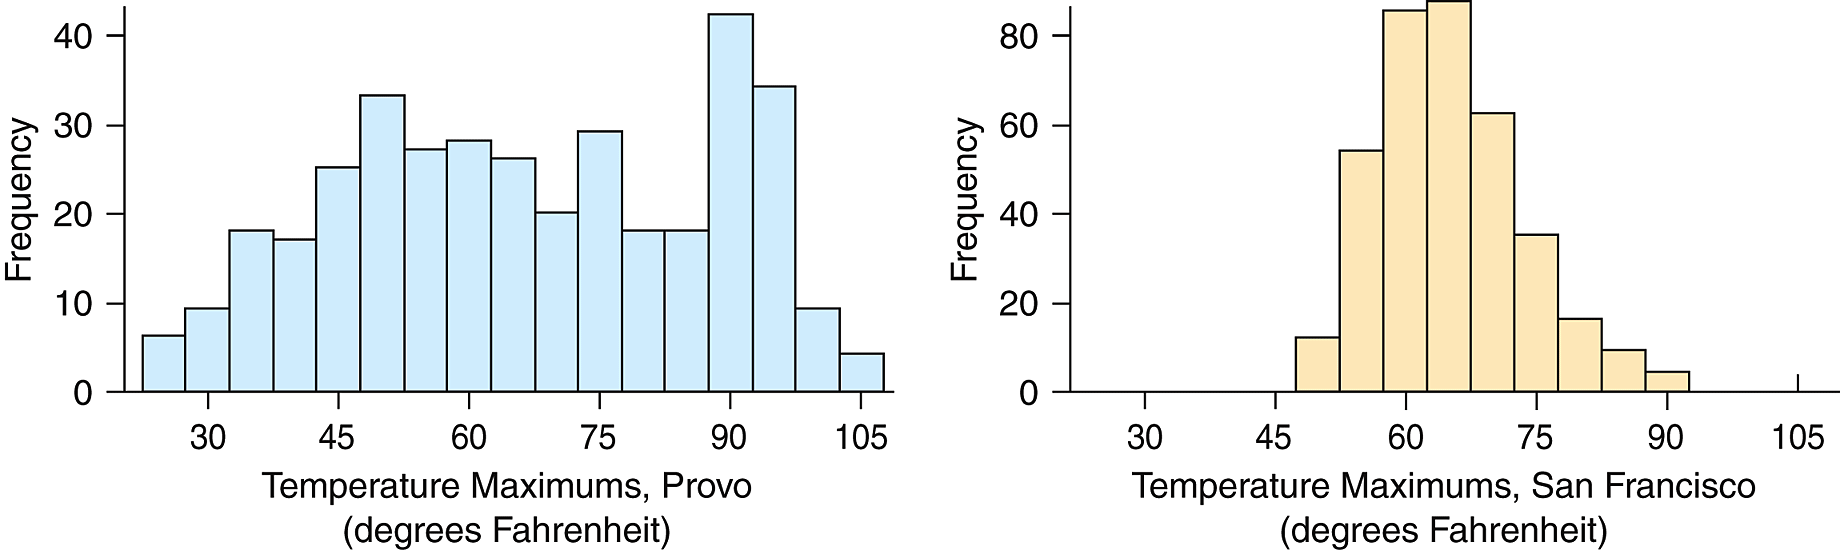
\includegraphics[width=0.8\linewidth]{images/math211_figure_3p7}
  \end{center}
  \vspace*{\stretch{1}}

  \begin{ex*}
    Below are three histograms representing distributions with the same mean. Which distribution has the largest standard deviation? Which has the smallest?
  \end{ex*}
  \begin{center}
    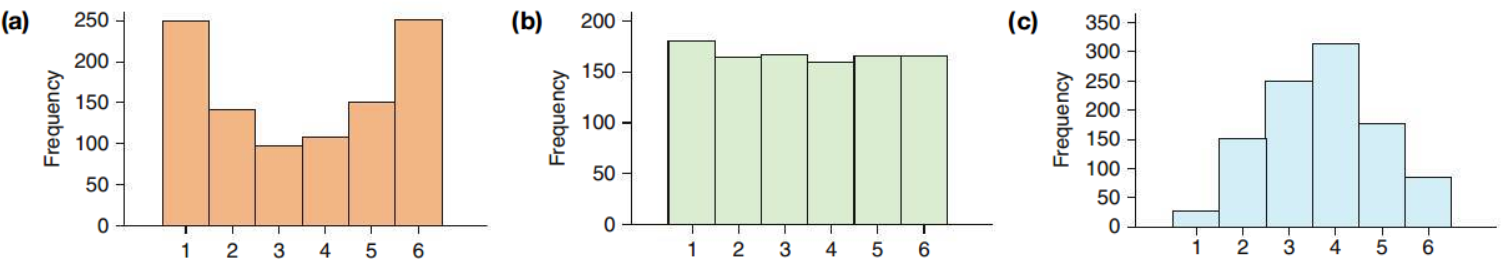
\includegraphics[width=0.95\linewidth]{images/math211_figure_3p8}
  \end{center}
  \vspace*{\stretch{1}}
  \pagebreak

  \begin{ex*}
    Recall the data set of gas prices from before. Use StatCrunch to compute the standard deviation of this data set and interpret the result:
    \hspace*{\stretch{1}}\href[pdfnewwindow]{https://www.statcrunch.com/}{\textcolor{blue}{\underline{statcrunch.com}}}

  \end{ex*}
  \begin{center}
    \begin{tabular}{@{}*{4}{c}@{}}\toprule
      \$2.19 & \$2.19 & \$2.39 & \$2.19 \\
      \$2.24 & \$2.39 & \$2.27 & \$2.29 \\
      \$2.17 & \$2.29 & \$2.30 & \$2.29 \\\bottomrule
    \end{tabular}
  \end{center}
  \begin{enumerate}
    \item Click ``Open StatCrunch''
    \item Enter data into spreadsheet
    \item Under the ``Stat'' menu, select ``Summary Stats'' then ``Columns'' or ``Rows''
  \end{enumerate}
  \vspace*{\stretch{1}}
  \begin{defn*}
    The \textbf{variance} is the standard deviation squared:
      \[s^2=\frac{\sum \parens{x_i-\bar{x}}^2}{\nmo}\]
    \vspace*{-\baselineskip}
  \end{defn*}

  \pagebreak
\end{document}
